% UTF-8
% XeLaTeX
\documentclass[a4paper,10.5pt]{article}
\usepackage[left=2.2cm,right=2.2cm,top=2.5cm,bottom=2.2cm]{geometry}
\usepackage[BoldFont,SlantFont]{xeCJK}
\usepackage[colorlinks,CJKbookmarks,urlcolor=blue,linkcolor=red,backref=page]{hyperref}
\usepackage{indentfirst}
\usepackage{graphicx}
\usepackage{xcolor}
\usepackage{caption}
\usepackage{tikz}
\usepackage{mathrsfs}
\usepackage{amsmath}
\usepackage{amssymb}
\DeclareSymbolFont{EulerExtension}{U}{euex}{m}{n}
\DeclareMathSymbol{\euintop}{\mathop} {EulerExtension}{"52}
\DeclareMathSymbol{\euointop}{\mathop} {EulerExtension}{"48}
\let\intop\euintop
\let\ointop\euointop
\usetikzlibrary{arrows}
\usetikzlibrary{backgrounds}
\renewcommand{\tablename}{表}
\renewcommand{\figurename}{图}
\captionsetup[table]{labelsep=space}
\captionsetup[figure]{labelsep=space}
\newcommand\md {\mathrm{d}}
\newcommand\ml {\mathscr{L}}
\linespread{1.1}
\setmainfont{Times New Roman}
\setCJKmainfont{Adobe Song Std}
\setCJKfamilyfont{KaiTi}{KaiTi}
\newcommand \kaiti {\CJKfamily{KaiTi}}
\setCJKfamilyfont{Adobe Heiti Std}{Adobe Heiti Std}
\newcommand \heiti {\CJKfamily{Adobe Heiti Std}}
\title{\heiti 单速一维均匀裸平板堆$\boldsymbol{S_{N}}$模拟的MATLAB实现}
\author{\href{mailto:sunxb10@gmail.com}{孙晓博}\\2010011732\\{}工物系核01班}
\date{}
\begin{document}
\maketitle
{\kaiti 主要参考了杜书华《输运问题的计算机模拟》(湖南科学技术出版社)及胡永明《反应堆物理数值计算方法》(国防科技大学出版社),修改了书中的下标表述法以适应MATLAB编程。}\par
\section{待解题目}
单速一维均匀裸平板堆,堆半厚度$a_{0}=66.0053\,\mathrm{cm}$,两侧为真空边界条件,$\Sigma_{t}=0.050/\mathrm{cm}$,$\Sigma_{s}=0.030/\mathrm{cm}$,$\nu\Sigma_{f}=0.0225/\mathrm{cm}$。\par
\section{算法原理}
一维平板输运微分方程的守恒形式:
\begin{align}
\mu\frac{\partial\Phi(x,\mu)}{\partial{}x}+\Sigma_{t}\Phi(x,\mu)=S(x)\label{eq:diff_eq}
\end{align}
其中角度$\mu$按照Gauss-Legendre求积法离散为$\mu_{m}$ ($m=1,2,\cdots,N$),相应的权重为$\omega_{m}$。只需考虑右半侧平板,坐标$x$离散为$x_{2k}$ ($k=1,2,\cdots,K$),其中$K$ 为所取的网格数,在坐标节点的两侧和中间插入中间节点$x_{2k'+1}$ ($k'=0,1,2\cdots,K$),其中$x_{1}=0$,$x_{2K+1}=a_{0}$。相应节点处中子角注量率记为$\Phi_{2k,m}$ 或$\Phi_{2k'+1,m}$。\par
如上离散操作得到空间网格$\Delta_{2k}=x_{2k+1}-x_{2k-1}$,在网格内积分得到差分格式的输运方程
\begin{align}
\mu_{m}(\Phi_{2k+1}-\Phi_{2k-1})+\Delta_{2k}\Sigma_{t}\Phi_{2k,m}=\Delta_{2k}S_{2k}\label{eq:delta_eq}
\end{align}
其中
\begin{align*}
\Phi_{2k,m}&=\frac{1}{\Delta_{2k}}\int_{x_{2k-1}}^{x_{2k+1}}\Phi_{m}(x)\md{}x\\
S_{2k}&=\frac{1}{\Delta_{2k}}\int_{x_{2k-1}}^{x_{2k+1}}S(x)\md{}x
\end{align*}
\par
边界条件:平板外侧真空,平板中央对称
\begin{align}
\Phi_{2K+1,m}&=0\quad(\mu_{m}<0)\label{eq:outer_boundary}\\
\Phi_{1,m}&=\Phi_{1,N+1-m}\label{eq:inner_boundary}
\end{align}
\par
接下来即可考虑求解\eqref{eq:delta_eq}式,首先在做空间离散时可以取等距节点,使$\Delta_{2}=\Delta_{4}=\cdots=\Delta_{2k}=\Delta$。之后处理源项,由Gauss-Legendre 求积法可得
\begin{align}
S_{2k}&=\frac{\Sigma_{s}+\nu\Sigma_{f}}{2}\sum_{m=1}^{N}\left(\Phi_{2k,m}\cdot\omega_{m}\right)
\end{align}
由步函数格式可得
\begin{align}
\Phi_{2k,m}=\frac{1}{2}\left(\Phi_{2k+1,m}+\Phi_{2k-1,m}\right)\label{eq:step_func}
\end{align}
\par
对于$\mu_{m}<0$的情况,先由外表面边界条件\eqref{eq:outer_boundary}式得到$\Phi_{2K+1,m}=0$,之后由\eqref{eq:delta_eq}式可得
\begin{align}
\Phi_{2k-1,m}=\frac{2+\ml_{m}}{2-\ml_{m}}&\cdot\Phi_{2k+1,m}-\frac{2\ml_{m}}{2-\ml_{m}}\cdot\frac{S_{2k}}{\Sigma_{t}}\label{eq:mu<0-iter}\\
k&=K,K-1,\cdots,1\notag\\
m&=1,2,\cdots,\frac{N}{2}\notag
\end{align}
其中$\ml_{m}=\Sigma_{t}\cdot\Delta/\mu_{m}$,再加上\eqref{eq:step_func}式可算出所有$\mu_{m}<0$的节点。
\par
对于$\mu_{m}>0$的情况,先由中央边界条件\eqref{eq:inner_boundary}式得到$\Phi_{1,m}$,之后由\eqref{eq:delta_eq}式可得
\begin{align}
\Phi_{2k+1,m}=\frac{2-\ml_{m}}{2+\ml_{m}}&\cdot\Phi_{2k-1,m}-\frac{2\ml_{m}}{2+\ml_{m}}\cdot\frac{S_{2k}}{\Sigma_{t}}\label{eq:mu>0-iter}\\
k&=1,2,\cdots,K\notag\\
m&=\frac{N}{2}+1,\frac{N}{2}+2,\cdots,N\notag
\end{align}
其中$\ml_{m}=\Sigma_{t}\cdot\Delta/\mu_{m}$,再加上\eqref{eq:step_func}式可算出所有$\mu_{m}>0$的节点。\par
\vspace{0.5cm}
作为简单的示例,$N=4$、$K=4$时的网格节点迭代求解顺序如图\ref{fg:node_seq}所示。
\begin{figure}[htbp]
\centering
\begin{tikzpicture}[show background rectangle,background rectangle/.style={fill=blue!10!white}]
\draw[->,>=stealth,thick] (-3,0) -- (4,0);
\draw (3.8,0.3) node[anchor=west] {$\mu$};
\draw[->,>=stealth,thick] (0,0) -- (0,9);
\draw (-0.1,8.7) node[anchor=east] {$x$};
\foreach \j in {1,3,...,7}
{
    \foreach \i in {-3,-1}
    {
        \draw[->,>=angle 45,red,thick] (\i,\j+0.9) .. controls (\i+0.5,\j) .. (\i,\j-0.9);
        \draw[->,>=angle 45,green!70!black,thick] (\i,\j+0.9) -- (\i,\j+0.1);
        \draw[->,>=angle 45,green!70!black,thick] (\i,\j-0.9) -- (\i,\j-0.1);
    }
    \foreach \i in {1,3}
    {
        \draw[->,>=angle 45,densely dashed,red,thick] (\i,\j-0.9) .. controls (\i+0.5,\j) .. (\i,\j+0.9);
        \draw[->,>=angle 45,green!70!black,thick] (\i,\j+0.9) -- (\i,\j+0.1);
        \draw[->,>=angle 45,green!70!black,thick] (\i,\j-0.9) -- (\i,\j-0.1);
    }
}
\draw[->,>=angle 45,teal,thick] (-3,-0.8) .. controls (-2,-2) and (2,-2) .. (3,-0.8);
\draw[->,>=angle 45,teal,thick] (-1,-0.8) .. controls (-0.6,-1.6) and (0.6,-1.6) .. (1,-0.8);
\foreach \i/\xtext in {-3/\mu_{1},-1/\mu_{2}}
{
    \filldraw[fill=yellow,draw=black,semithick] (\i-0.1,-0.1) rectangle ++(0.2,0.2);
    \filldraw[fill=green,draw=black,semithick] (\i-0.1,7.9) rectangle ++(0.2,0.2);
    \draw (\i,-0.3) node[anchor=north] {$\xtext$};
}
\foreach \i/\xtext in {1/\mu_{3},3/\mu_{4}}
{
    \filldraw[fill=blue,draw=black,semithick] (\i-0.1,-0.1) rectangle ++(0.2,0.2);
    \filldraw[fill=lightgray!50!white,draw=black,semithick] (\i-0.1,7.9) rectangle ++(0.2,0.2);
    \draw (\i,-0.3) node[anchor=north] {$\xtext$};
}
\foreach \j in {2,4,6}
{
    \foreach \i in {-3,-1,...,3}
    {
        \filldraw[fill=yellow,draw=black,semithick] (\i-0.1,\j-0.1) rectangle ++(0.2,0.2);
    }
}
\foreach \i in {-3,-1,1,3}
{
    \foreach \j in {1,3,5,7}
    {
        \filldraw[fill=darkgray,draw=black,semithick] (\i,\j) circle (0.1);
    }
}
\foreach \j/\ytext in {0/x_{1},1/x_{2},2/x_{3},3/x_{4},4/x_{5},5/x_{6},6/x_{7},7/x_{8},8/x_{9}}
{
    \draw (-3.2,\j) node[anchor=east] {$\ytext$};
}
\foreach \j/\ytext in {0,8/a_{0}}
{
    \draw (-3.8,\j) node[anchor=east] {$\ytext$};
}
\draw (-4.5,-2) node[anchor=west] {\textbf{图例:}};
\draw[->,>=angle 45,green!70!black,thick] (-4,-2.5) -- (-3,-2.5) node[anchor=west] {\textcolor{black}{应用\eqref{eq:step_func}式递推}};
\draw[->,>=angle 45,red,thick] (-4,-2.9) -- (-3,-2.9) node[anchor=west] {\textcolor{black}{应用\eqref{eq:mu<0-iter}式递推}};
\draw[->,>=angle 45,densely dashed,red,thick] (-4,-3.3) -- (-3,-3.3) node[anchor=west] {\textcolor{black}{应用\eqref{eq:mu>0-iter}式递推}};
\draw[->,>=angle 45,teal,thick] (-4,-3.7) -- (-3,-3.7) node[anchor=west] {\textcolor{black}{中央对称边界}};
\filldraw[thick,fill=darkgray,draw=black] (0.5,-2.5) circle(0.1) node[anchor=west] {$\quad$\textcolor{black}{实际的网格节点}};
\filldraw[fill=yellow,draw=black,semithick] (0.4,-3.0) rectangle ++(0.2,0.2) ++(-0.1,-0.1) node[anchor=west] {$\quad$\textcolor{black}{需要计算的中间节点}};
\filldraw[fill=lightgray!50!white,draw=black,semithick] (0.4,-3.4) rectangle ++(0.2,0.2) ++(-0.1,-0.1) node[anchor=west] {$\quad$\textcolor{black}{不需计算的中间节点}};
\filldraw[fill=green,draw=black,semithick] (0.4,-3.8) rectangle ++(0.2,0.2) ++(-0.1,-0.1) node[anchor=west] {$\quad$\textcolor{black}{外表面边界条件}};
\filldraw[fill=blue,draw=black,semithick] (0.4,-4.2) rectangle ++(0.2,0.2) ++(-0.1,-0.1) node[anchor=west] {$\quad$\textcolor{black}{中央边界条件}};
\end{tikzpicture}
\caption{$\ $迭代求解顺序($N=4$,$K=4$)}
\label{fg:node_seq}
\end{figure}
\par
程序算出中子角通量后即可根据Gauss-Legendre求积法得到中子通量密度
\begin{align}
\varphi_{2k}=\sum_{m=1}^{N}\left(\Phi_{2k,m}\cdot\omega_{m}\right)
\end{align}
\par
为避免负通量的出现和扩散,本程序使用了最简单的置零修正,即在迭代计算过程中反复检查,只要出现某点通量为负则立即将其置零。\par
由于采用了特殊的下标表述,因而程序的内存开销大于实际需要,比如$S$、$k_\mathrm{eff}$等矩阵有一半以上的元素为空,这也是将来程序优化时必须改进的一点。
\section{求解结果}
程序及报告已同步至\href{https://github.com/sunxb10/One-Dimensional-SN}{GitHub}网站。\par
程序取$N=8$,$K=400$,迭代中有效增值系数$k_{\mathrm{eff}}$相对误差上限为$10^{-8}$。程序共进行$57$轮循环,耗时$1.70\,\mathrm{s}$,编程测试平台:Intel$ {}^{\textregistered}$ Core${}^{\mathrm{TM}}$ i5-2410M CPU @ 2.30GHz (Sandy Bridge)、8GB RAM (DDR3-1333MHz)、Windows 7 Enterprise (64-bit)、MATLAB R2012b (64-bit)。\par
计算得到所有节点的平均有效增殖系数为$0.99991145$,其中最大有效增殖系数为$0.99991147$,最小有效增殖系数为$0.99991143$。\par
按照杜书华《输运问题的计算机模拟》一书中的理论,本题的截面数据相当于$C=(\Sigma_{s}+\nu\Sigma_{f})/\Sigma_{t}=1.05$,本题的半厚度相当于$a_{0}=3.3002650\lambda$ (其中$\lambda=1/\Sigma_{t}$为中子自由程),查阅《输运问题的计算机模拟》第148页表4.5.1给出的$C=1.05$时的临界半厚度值,可知本题所给的条件与临界条件($a_{0}=3.3002638\lambda$)非常接近,因此算出有效增殖系数非常接近于$1$是合理的。\par
以《输运问题的计算机模拟》第149页表4.5.3给出的$C=1.05$时的中子通量分布为标准值,对程序计算结果做校验,结果如表\ref{tb:01}所示。\par
\begin{table}[htbp]
\centering
\caption{$\quad$中子通量分布校验结果(球心通量归一)}
\label{tb:01}
\begin{tabular}{c|c|c|c|c}
\hline
& \multicolumn{4}{|c}{校验点$x/a_{0}$}\\
\cline{2-5}
& 0.25 & 0.50 & 0.75 & 1.00\\
\hline
\textbf{计算值} & 0.94756412 & 0.79436289 & 0.55409599 & 0.21662752\\
\hline
\textbf{标准值} & 0.94714400 & 0.79372641 & 0.55329025 & 0.21419206\\
\hline
\end{tabular}
\end{table}
计算得到的中子注量率分布如图\ref{fg:phi-rate-dist}所示。
\begin{figure}[htbp]
\centering
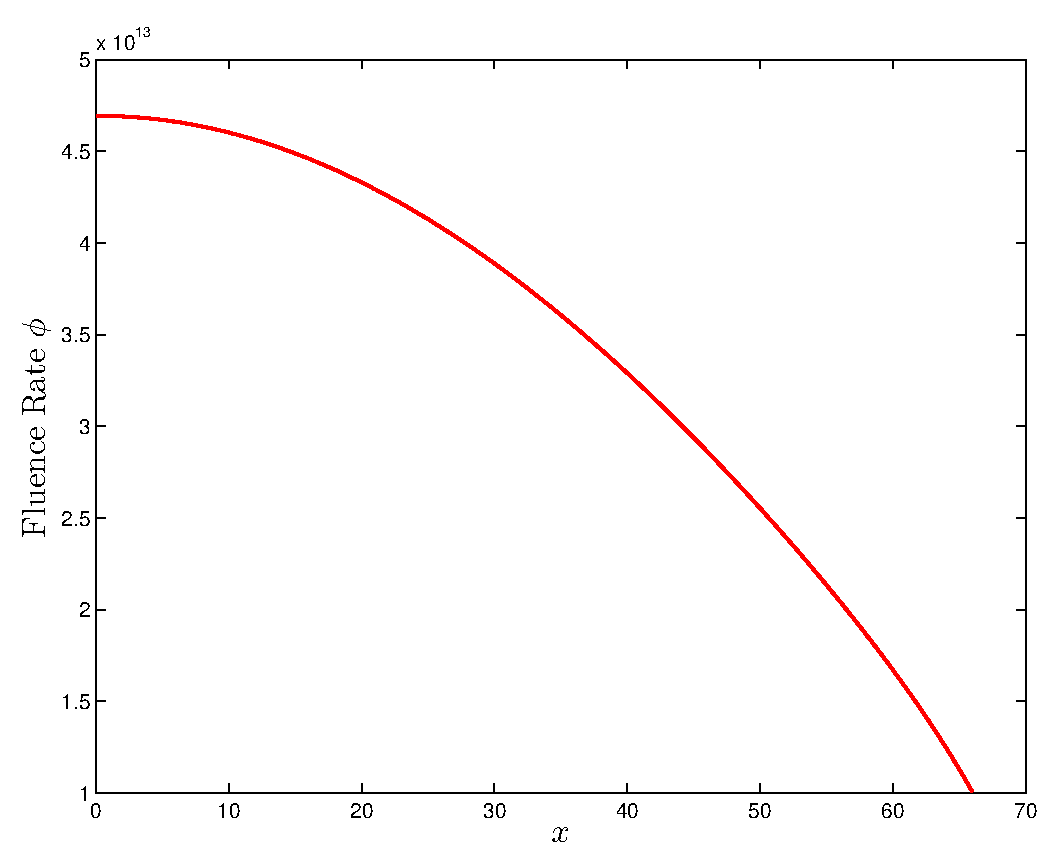
\includegraphics[width=0.7\textwidth]{1D_plane_neutron_flux.eps}
\caption{$\quad$中子注量率分布($N=8$,$K=400$)}
\label{fg:phi-rate-dist}
\end{figure}
\end{document}
